\section{Исследовательская часть}

\subsection{Цель исследования}

Целью исследования является сравнение производительности программного обеспечения с использованием кеширования в in-memory СУБД и без него.

Задачи, требуемые для достижения цели:

\begin{itemize}[leftmargin=1.6\parindent]
	\item реализовать кеширование ответов на уровне приложения;
	\item наполнить базу данных тестовыми данными;
	\item провести нагрузочное тестирование с кешированием и без кеширования с постоянным и линейным профилем нагрузки;
	\item сравнить полученные результаты и сформулировать вывод.
\end{itemize}

\subsection{Описание исследования}
Для оптимизации запросов в приложении было реализовано кеширование ответов. Система проверяет аргументы каждого запроса и ищет соответствующий ответ в кеше. Если ответа нет, то данные запрашиваются из базы данных, сохраняются в кеш и отдаются пользователю. Повторный запрос будет обработан быстрее, так как данные уже есть в кеше и запрос в базу данных не требуется. 

В роли кеша будет использоваться in-memory СУБД redis. Для генерации нагрузки и сбора метрик будет использоваться Yandex.Tank\cite{yandex-tank}.

Для анализа полученных метрик  будет использоваться  инструмент анализа производительности веб-приложений Overload\cite{overload}.

Для тестирования была выбрана конечная точка  $/user/\{user\_id\}/projects$ с параметром $user\_id$ равным идентификатору пользователя, этот параметр находится в интервале от 1 до 10.  

Набор тестовых данных включал в себя 10 пользователей и 10000 проектов. Данные были сгенерированы с помощью скрипта на языке python \cite{python} и библиотеки faker \cite{faker}.

\newpage
В листинге \ref{lst:tank-ammo} представлен список выполняемых запросов для тестирования.

\begin{code}
	\captionof{listing}{Примеры запросов для нагрузочного тестирования}
	\label{lst:tank-ammo}
	\inputminted
	[
	frame=single,
	framerule=0.5pt,
	framesep=20pt,
	fontsize=\footnotesize,
	tabsize=4,
	linenos,
	numbersep=5pt,
	xleftmargin=10pt,
	firstline=1,
	lastline=27,
	]
	{text}
	{lst/ammo.txt}
\end{code}

\subsection*{Технические характеристики}
Технические характеристики устройства, на котором выполнялось тестирование, следующие.

\begin{itemize}
	\item Операционная система: macOS 12.5.1.
	\item Память: 16 ГБ.
	\item Процессор: Intel® Core™ i7-1068NG7  CPU @ 2.30ГГц \cite{intel}.
\end{itemize}

Исследование проводилось на ноутбуке, включенном в сеть электропитания. Во время экспериментов ноутбук был нагружен только встроенными приложениями окружения, а также непосредственно системой тестирования.

\newpage
\subsection{Результаты исследования}

Ниже представлены графики зависимости времени ответа конечной точки от количества запросов в секунду (rps) при линейной и постоянной нагрузке. 

Графики включают в себя три метрики: rps, avg, и 98-й квантиль времени ответа, где 
rps - это количество запросов в секунду направленных на конечную точку,
avg -- среднее время ответа конечной точки.


\subsubsection*{Линейная нагрузка}

График времени  ответа конечной точки при линейной
нагрузке без использования кеширования представлен на рисунке \ref{fig:lin-bench-no-cache}.


\begin{figure}[hbtp]
	\centering
	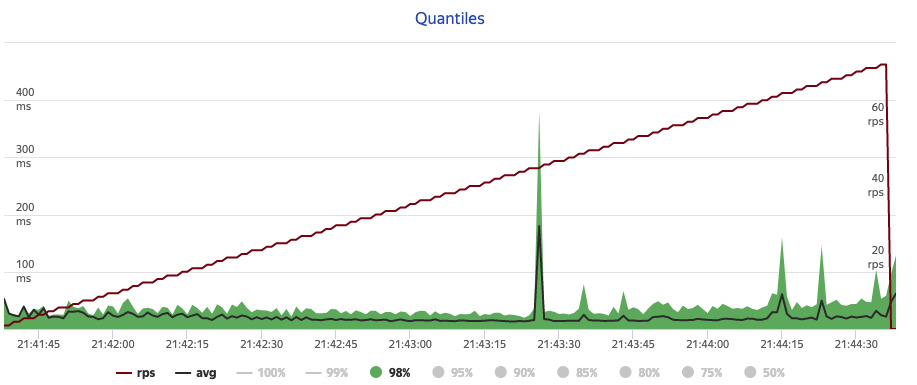
\includegraphics[width=\textwidth]{img/bench-lin-no-cache}
	\caption{График времени ответа конечной точки при линейной нагрузке без использования кеширования}
	\label{fig:lin-bench-no-cache}
\end{figure}

\newpage

График  времени ответа конечной точки при линейной
нагрузке с использованием кеширования представлен на рисунке \ref{fig:lin-bench-cache}.

\begin{figure}[hbtp]
	\centering
	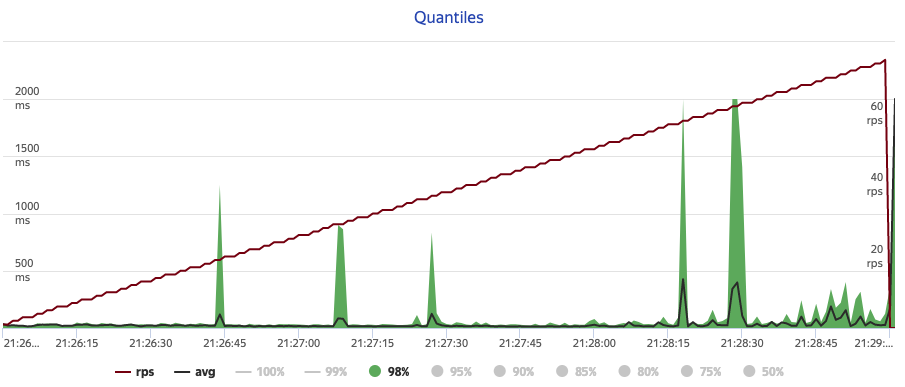
\includegraphics[width=\textwidth]{img/bench-lin-cache}
	\caption{График времени ответа конечной точки при линейной нагрузке с использованием кеширования}
	\label{fig:lin-bench-cache}
\end{figure}

Исследование с помощью линейной нагрузки показало, что кеширование не приводит к росту производительности, наоборот, появляются частые "скачки"\ времени ответа.


\subsubsection*{Постоянная нагрузка}

График  времени ответа конечной точки при постоянной
нагрузке без использования кеширования представлен на рисунке \ref{fig:post-bench-no-cache}.

\begin{figure}[hbtp]
	\centering
	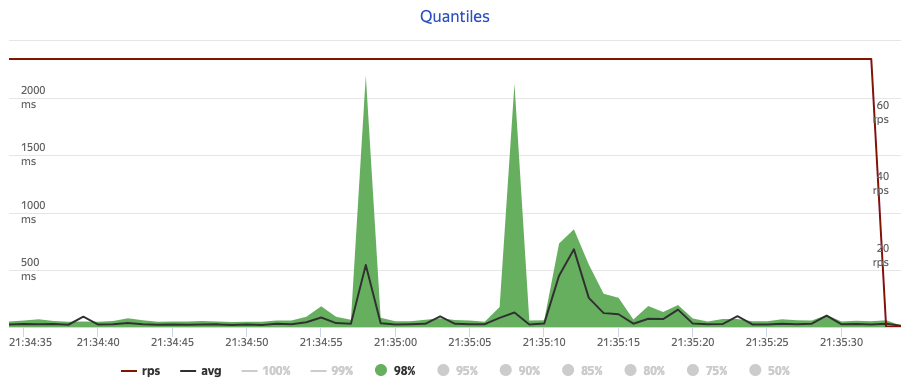
\includegraphics[width=\textwidth]{img/bench-post-no-cache}
	\caption{График времени ответа конечной точки при постоянной нагрузке без использования кеширования}
	\label{fig:post-bench-no-cache}
\end{figure}

\newpage

График  времени ответа конечной точки при постоянной
нагрузке с использованием кеширования представлен на рисунке \ref{fig:post-bench-no-cache}.

\begin{figure}[hbtp]
	\centering
	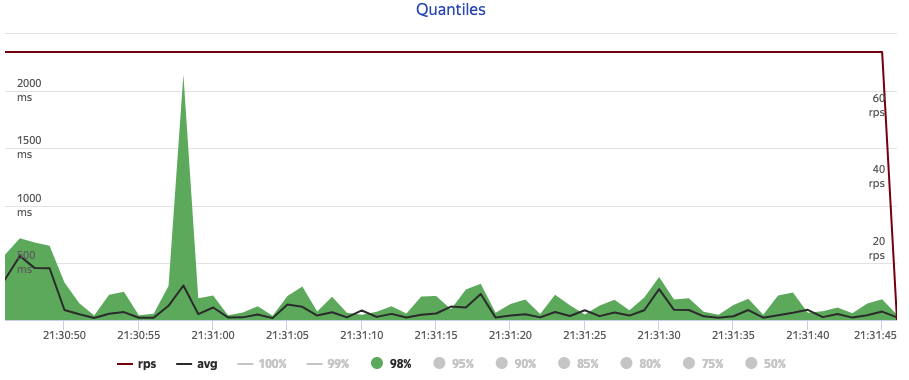
\includegraphics[width=\textwidth]{img/bench-post-cache}
	\caption{График времени ответа конечной точки при постоянной нагрузке c использованием кеширования}
	\label{fig:post-bench-cache}
\end{figure}

Исследование с помощью постоянной нагрузки(75 запросов в секунду) показало, что кеширование работает быстрее с момента, когда все данные попали в кеш. Общий 99-й квантиль времени ответа без кеширования -- 760 мс. С кешированием -- 660 мс. Также на графиках видно, что "скачков"\ времени ответа без использования кеширования больше, чем с его использованием.

\subsection*{Вывод}

В данном разделе было проведено исследование, в ходе которого было реализовано кеширование ответов приложения конечной точки \\$/user/\{user\_id\}/projects$.

Исследование показало, что при линейной нагрузке кеширование приводит к частым "скачкам"\ времени ответа сервиса, а при постоянной нагрузке(75 запросов в секунду) наоборот -- к уменьшению времени ответа на 15\%. 

Использование кеширования в системе может повысить производительность конечной точки при постоянной нагрузке. Однако, кеширование должно быть применено только к конечным точкам, которые имеют высокий коэффициент попадания запросов в кеш. В противном случае, применение кеширования не приведет к повышению производительности, поскольку система будет сначала проверять наличие необходимых данных в кеше, а только потом - в базе данных.





\pagebreak